\chapter{Implementação}\label{chap:implement}

\section*{}

Neste capítulo é especificado de forma detalhada o desenvolvimento e implementação do protótipo desenvolvido, bem como as suas principais características. Pretende-se apresentar as várias fases de desenvolvimento e, em cada uma delas, o trabalho realizado e as conclusões retiradas tendo em vista uma melhoria constante do produto final.

\section{Especificação de Requisitos}

Para desenvolver uma aplicação que se adequasse às necessidades reais dos utilizadores e das entidades envolvidas, foi necessário analisar o sistema de bilhética atual e perceber quais as ações fundamentais para uma implementação eficaz. Para além disso, foi também necessário avaliar quais as principais funcionalidades que trariam valor ao serem implementadas e que tirariam o máximo proveito das capacidades dos dispositivos móveis. Em anexo encontra-se a especificação detalhada dos requisitos funcionais. Ver Anexo~\ref{rer}.

\subsection{Requisitos Funcionais}

Começando pelos requisitos relacionados com a utilização de autenticação de utilizadores, salvaguardando assim os dados pessoais e permitindo a segurança das operações efetuadas, definiram-se como requisitos funcionais os seguintes:
\begin{itemize}
\item O sistema deve permitir o registo de um novo utilizador;
\item O sistema deve permitir a autenticação de um utilizador já registado;
\item O sistema deve permitir a um utilizador autenticado alterar os seus dados pessoais;
\item O sistema deve permitir a um utilizador autenticado terminar a sessão ativa.
\end{itemize}

Os requisitos funcionais relacionados com o funcionamento de um sistema de bilhética são os seguintes:
\begin{itemize}
\item O sistema deve permitir a compra de títulos por utilizadores autenticados;
\item O sistema deve utilizar os fornecedores de localização do dispositivo móvel para identificar a paragem onde o utilizador autenticado se encontra;
\item O sistema deve permitir ao utilizador autenticado a escolha manual da paragem de entrada;
\item O sistema deve listar as linhas e respetivos sentidos que passam na paragem selecionada pelo utilizador autenticado;
\item O sistema deve permitir ao utilizador autenticado escolher o título a validar, apresentando todos os títulos disponíveis que se adequem à paragem e linha selecionadas;
\item O sistema deve permitir ao utilizador autenticado efetuar a validação do título escolhido, apresentando a paragem limite até à qual pode viajar;
\item O sistema deve permitir a mudança de linha (transbordo), quando existir um título válido;
\item O sistema deve permitir a confirmação da validade do título em utilização, por parte do revisor.
\end{itemize}

Por fim, os requisitos funcionais relacionados com a visualização de informação por parte do utilizador:
\begin{itemize}
\item O sistema deve permitir a consulta do estado atual do título validado;
\item O sistema deve permitir o acesso ao histórico de operações efetuadas pelo utilizador autenticado;
\item O sistema deve permitir o acesso ao histórico de validações realizadas pelo utilizador autenticado;
\item O sistema deve permitir a consulta do saldo de títulos disponíveis;
\item O sistema deve permitir a consulta de saldo da carteira virtual.
\end{itemize}

\subsection{Requisitos Não Funcionais}

Para além dos requisitos acima especificados, foram também delineadas algumas características que a aplicação deve conter:
\begin{itemize}
\item Comunicação - É necessário uma ligação à rede com um acesso estável e com uma largura de banda mínima, que permita a plena utilização de todas as funcionalidades disponíveis;
\item Eficiência - Uma normal utilização do sistema requer inúmeros acessos simultâneos à aplicação e, consequentemente, à sua base de dados. Logo, é fulcral que a aplicação esteja estruturada para que a informação seja acedida e apresentada em tempos de resposta mínimos, de modo a que o utilizador veja satisfeitos os seus propósitos de manipulação de informação;
\item Fiabilidade - O sistema deverá garantir a integridade dos dados submetidos;
\item Manutenção - O sistema deverá permitir uma fácil manutenção e adição de novas funcionalidades;
\item Segurança - O sistema deve estar devidamente protegido para que não haja a possibilidade de acessos indevidos a dados confidenciais dos utilizadores.
\item Usabilidade - Pretende-se que a interface da aplicação seja intuitiva e de fácil utilização, para que o utilizador não perca muito tempo no processo de aprendizagem do manuseamento da mesma. É importante também que o número de cliques para execução das ações seja o menor possível, reduzindo assim o tempo de execução. O sistema deverá, também, oferecer mensagens de erro claras e ajuda contextual;
\item Compatibilidade - O sistema deverá funcionar perfeitamente em dispositivos Android com verão 2.2 (API 8) ou superior. Para além disso, o sistema deverá ter uma integração coerente com a aplicação MOVE-ME.
\end{itemize}

\section{Principais Casos de Uso}

\subsection{Compra}

O primeiro passo a realizar, tal como acontece hoje em dia, é a compra de títulos de viagem. Esta compra pode ser feita de forma simples, selecionando a modalidade desejada, configurando-a (número de zonas e quantidade no caso dos títulos Ocasionais e Andante 24; escolha de zonas no caso da Assinatura) e finalizando a compra após confirmação dos detalhes.
\\Os preços utilizados são exatamente os mesmos em vigor nos postos de venda tradicionais e, tal como acontece atualmente, na compra de 10 títulos ocasionais ou Andante 24, é oferecido um título extra com a mesma tipologia.
\\Baseado no sistema Andante, a assinatura pode ser comprada desde o dia 16 do mês anterior até ao dia 15 do mês corrente. Como tal, caso o utilizador não compre a assinatura até ao dia 15, terá de viajar o resto do mês com títulos ocasionais. Apenas poderá comprar a assinatura para o mês seguinte, tal como acontece nos postos de venda tradicionais.
\\Para além de ser apresentado o saldo atual da carteira virtual, o utilizador consegue facilmente visualizar quais os títulos que tem disponíveis e saber assim se tem ou não necessidade de comprar um novo título.

\subsection{Validação}

Para poder viajar nos veículos de transportes públicos, o utilizador deve proceder à validação de um dos títulos disponíveis. Para tal deve, de antemão, garantir que possui o título necessário para a viagem que vai realizar.
\\Antes de realizar a validação do título é necessário selecionar a paragem e linha de entrada. A aplicação tenta, de forma automática, calcular a posição do utilizador e apresentar as paragens encontradas num raio de 80 metros, permitindo assim uma margem de erro de cálculo. No entanto, caso não seja possível calcular a posição atual do utilizador ou esta seja errada, é possível uma introdução manual da paragem, escolhendo o operador, a linha e finalmente a paragem.
\\Após a escolha da paragem são listadas todas as linhas que nela param, permitindo ao utilizador escolher aquela onde vai entrar.
\\Concluído o processo de validação, o utilizador pode viajar normalmente no veículo e será criada uma notificação no telemóvel que lhe indica o tempo restante e o título em uso. Para além disso, essa notificação permite aceder ao menu de fiscalização, caso solicitado pelo revisor.

\subsection{Consulta}

É importante também aceder ao estado atual da carteira de títulos e da carteira virtual. Muitas vezes os utilizadores deparam-se com o problema de estarem em casa e não saberem se têm títulos carregados para poder efetuar uma viagem, tendo de se deslocarem a um posto de venda para efetuar essa verificação. Isso muitas vezes implica a perda do veículo desejado ou alterações no planeamento diário.
\\A aplicação permite ao utilizador consultar em qualquer altura quais os títulos que tem disponíveis, bem como as operações que efetuou (carregamentos, compras, etc.). Para além disso permite-lhe ainda visualizar o histórico de validações efetuadas, separando os títulos ocasionais da assinatura, porque normalmente existe uma discrepância no número de validações dum tipo e doutro, sendo mais fácil a visualização em separado.

\section{Arquitetura}

A aplicação baseia-se numa arquitetura Servidor-Cliente tradicional, com utilização de uma base de dados de suporte local, mas que serve apenas para acelerar alguns processos, sendo sempre necessário comunicar ao servidor quaisquer alterações que sejam feitas.
\\A aplicação comunica com o servidor através de ligação à Internet, utilizando serviços \web com API própria. Alguns dos serviços em utilização são os mesmos que se encontram na aplicação MOVE-ME, pois fornecem informação pertinente para ambas as aplicações e também tendo em foco uma futura integração das duas. Ver Figura~\ref{fig:architecture}.

\begin{figure}[t]
  \begin{center}
    \leavevmode
    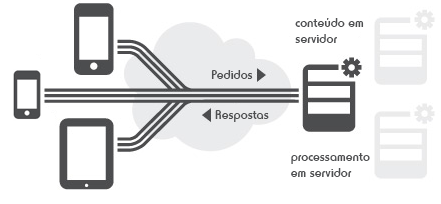
\includegraphics[scale=0.8]{architecture}
    \caption{Arquitetura Servidor-Cliente}
    \label{fig:architecture}
  \end{center}
\end{figure}

\section{Modelo Concetual}

Antes de desenvolver a aplicação é necessário ter presentes os conceitos envolvidos na mesma e a relação existente entre eles. A Figura~\ref{fig:class_diagram} apresenta o modelo concetual que serve de base à aplicação móvel, permitindo visualizar a multiplicidade das relações existentes entre classes, bem como os atributos específicos de cada classe.

\begin{figure}[t]
  \begin{center}
    \leavevmode
    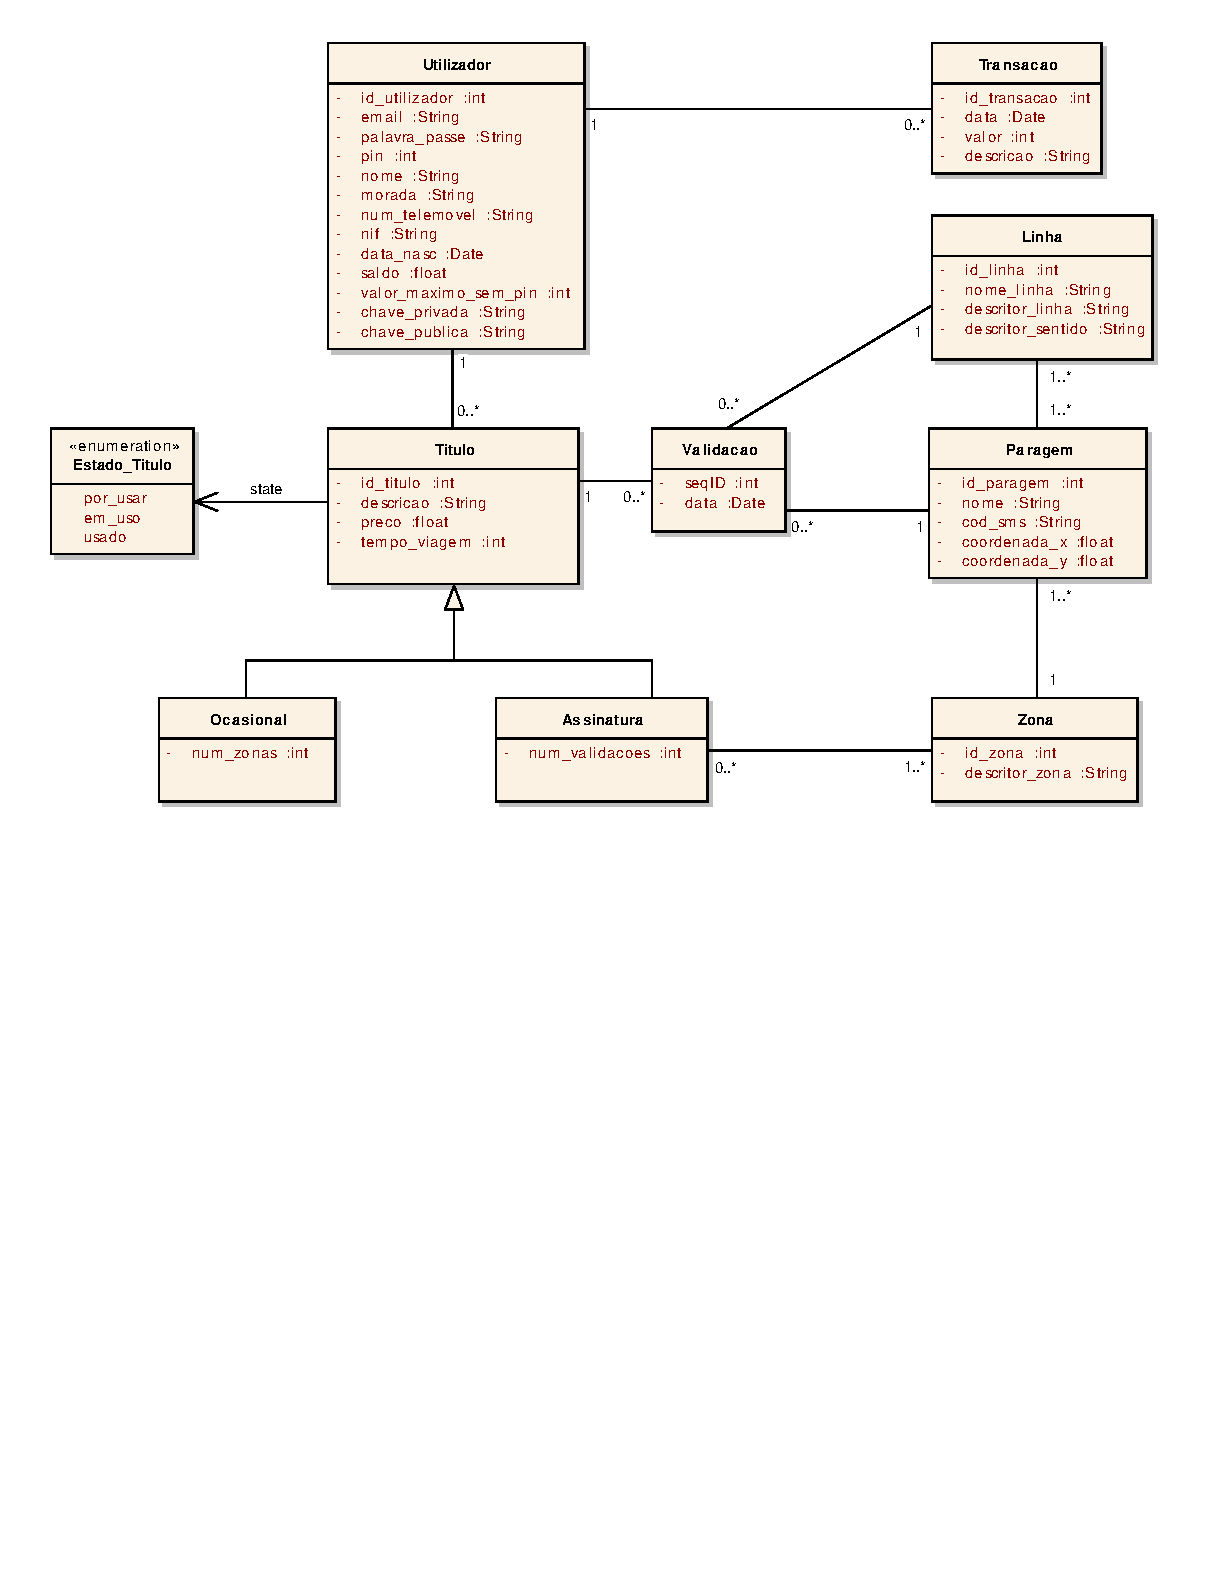
\includegraphics[scale=0.8]{class_diagram}
    \caption{Modelo Concetual}
    \label{fig:class_diagram}
  \end{center}
\end{figure}

\subsection{Utilizador}

Sendo uma aplicação de uso personalizado, é necessário associar toda a informação a um determinado utilizador. Para além dos dados pessoais do utilizador (nome, morada, número de telemóvel, Número de Informação Fiscal e data de nascimento), são também armazenados os dados de autenticação (endereço de correio eletrónico, palavra-passe e PIN numérico) e dados relacionados com a aplicação (saldo atual do utilizador e chaves de encriptação - pública e privada).
\\O elemento que garante a unicidade do utilizador é o endereço de correio eletrónico, pelo que após o registo, o utilizador não o poderá alterar. Por se tratar de um número único e invariável, também o Número de Identificação Fiscal não pode ser alterado através da aplicação, servindo para confirmação de identidade caso seja solicitado por parte do revisor.

\subsection{Título}

Os títulos são a componente central da aplicação, sendo que é através deles que se processam as principais funcionalidades da aplicação. Apesar de poder ser de diferentes tipos (Ocasional, Andante 24 e Assinatura Mensal), os diversos títulos possuem características em comum: descrição, preço e tempo de viagem. Para além disso, cada título tem associado a si um determinado estado (Por Usar, Em Uso ou Usado) e um conjunto de validações.

\subsubsection{Ocasional}

Em termos concetuais, o conceito ocasional engloba tanto os títulos de viagem como os títulos Andante 24, por se basearem no mesmo princípio: uso limitado durante um determinado período de tempo e pelo número de zonas estipulado na tipologia do título. A única diferença prende-se com o facto de num título ocasional o tempo de viagem ser calculado em função da tipologia enquanto que num título Andante 24 é sempre de vinte e quatro horas.
\\Para além dos atributos herdados, é também necessário saber o número de zonas permitidas durante a utilização do título.

\subsubsection{Assinatura}

A assinatura é o modelo mensal, com número ilimitado de utilizações dentro do mês estipulado e nas zonas previamente selecionadas. Para além disso, a assinatura é de uso pessoal e intransmissível.
\\Para disponibilizar alguma informação extra ao utilizador, é também guardado o número de validações. Pode ser utilizado, no futuro, para aconselhar o utilizador a utilizar títulos ocasionais caso o número de validações seja baixo, por exemplo.

\subsection{Validação}
Uma validação é o conceito que relaciona a utilização de um determinado título a uma paragem e linha, registando a data e hora, tendo associado um número sequencial único que serve para controlo por parte do revisor.

\subsection{Paragem}
Paragem é a localização física onde os veículos de determinadas linhas efetuam paragem, permitindo a entrada e saída de passageiros. Sendo uma das funcionalidades da aplicação, a apresentação das paragens mais próximas da localização do utilizador, é necessário saber as coordenadas de cada paragem, bem como a informação que a identifica unicamente.

\subsection{Linha}
Linha corresponde ao trajeto efetuado pelos veículos e que é constituído por diversas paragens. Para além de identificar unicamente cada linha é necessário distinguir também o sentido do trajeto, pois, em muitos casos, o percurso efetuado (e respetivas paragens) difere no sentido de ida e de volta.

\subsection{Zona}
Partindo da designação de zona do sistema Andante, é o conceito que permite ao utilizador identificar a tipologia do título a adquirir para determinada viagem. Cada paragem tem uma zona associada.

\subsection{Transação}
Uma transação é uma operação efetuada na aplicação que envolva movimentos monetários. Isto envolve tanto o carregamento da carteira virtual, como a compra de títulos. Este conceito é fundamental para permitir ao utilizador visualizar o histórico de operações efetuadas na aplicação.

\section{API}

A API utilizada na aplicação pode ser dividida em dois grupos: um especificamente desenvolvido para a aplicação e outro que é constituído por serviços que já são utilizados pela aplicação MOVE-ME. Para uma descrição detalhada da API ver Anexo~\ref{api}.

\subsection{API Comum}

\subsubsection{GetAllLinesPathsByStop}

Este serviço permite obter a listagem de linhas e respetivos trajetos que passam numa determinada paragem. Uma linha pode ter um ou mais trajetos. É utilizado quando o utilizador escolhe a paragem de entrada.

\subsubsection{GetAllNearStops}

Este serviço permite obter a listagem de paragens encontradas num determinado raio centrado nas coordenadas especificadas. É utilizado para obter as paragens mais próximas da localização atual do utilizador, quando este inicia o processo de validação.

\subsubsection{LoadStopsByWord}

Este serviço permite obter a listagem de paragens que contenham determinada palavra no nome ou no código SMS. É utilizado quando o utilizador seleciona manualmente a paragem de entrada.

\subsubsection{GetAllProvidersName}

Este serviço permite obter a listagem completa de operadores de transportes públicos que operam no sistema Andante. É utilizado quando o utilizador seleciona manualmente a paragem de entrada.

\subsubsection{GetAllLinesByProvider}

Este serviço permite obter a listagem completa de linhas que um determinado operador tem. É utilizado quando o utilizador seleciona manualmente a paragem de entrada.

\subsubsection{GetAllStopsByLine}

Este serviço permite obter a listagem completa de paragens que constituem determinada linha (em todos os trajetos da linha). É utilizado quando o utilizador seleciona manualmente a paragem de entrada.

\subsection{API Específica}

\subsubsection{login}

Este serviço permite verificar os dados de login introduzidos e confirmar/rejeitar a autenticação do utilizador. É utilizado quando o utilizador se autentica na aplicação quando esta não tem nenhuma conta ativa.

\subsubsection{newUser}

Este serviço permite criar um novo utilizador, verificando a existência do email, o elemento único identificativo. É utilizado quando o utilizador se regista na aplicação.

\subsubsection{addTicket}

Este serviço permite adicionar títulos ocasionais à conta de um determinado utilizador. É utilizado quando o utilizador compra títulos ocasionais.

\subsubsection{addSignature}

Este serviço permite adicionar uma assinatura mensal à conta de um determinado utilizador. É utilizado quando o utilizador compra assinatura mensal.

\subsubsection{addMoneyUser}

Este serviço permite adicionar saldo à carteira virtual. É utilizado quando a conta é carregada.

\subsubsection{editUser}

Este serviço permite editar os dados pessoais do utilizador. É utilizado quando o utilizador altera os seus dados pessoais nas definições da aplicação.

\subsubsection{validate}

Este serviço permite validar um título da carteira de títulos. É utilizado após a seleção da paragem de entrada, da linha e trajeto e do título a validar.

\subsubsection{getPrices}

Este serviço permite obter a listagem de preços das várias modalidades do sistema Andante. É utilizado quando o utilizador procede à compra de títulos.

\subsubsection{getUser}

Este serviço permite obter a informação pessoal de um determinado utilizador. É utilizado quando o utilizador pretende alterar os seus dados pessoais.

\subsubsection{getTickets}

Este serviço permite obter a listagem de títulos disponíveis de um determinado utilizador. É utilizado quando o utilizador pretende proceder a uma validação, ver o saldo atual de títulos ou proceder à compra dos mesmos.

\subsubsection{getAccountMovements}

Este serviço permite obter as transações efetuadas por um determinado utilizador. É utilizado quando o utilizador pretende consultar o histórico de operações realizadas na sua conta.

\subsubsection{getAccountValidations}

Este serviço permite obter a listagem de validações de um determinado utilizador. É utilizado quando o utilizador pretende consultar o histórico de validações da sua assinatura ou dos títulos ocasionais.

\subsubsection{getStopZone}

Este serviço permite saber qual a zona Andante de determinada paragem. É utilizado para saber se é possível utilizar a assinatura na paragem selecionada.

\section{MobiPag STCP}

Por estar inserida na iniciativa nacional Pagamentos Móveis - MobiPag \cite{cedt} e por a STCP ser a operadora de transportes públicos que está envolvida no desenvolvimento da aplicação, esta tomou a denominação MobiPag STCP, não sendo este o nome final. Uma possível denominação será Andante Mobile, baseando-se no facto de a aplicação pretender apresentar-se como um substituto (opcional) do cartão Andante.
Nesta secção é ilustrada e detalhada a organização e dinâmica da aplicação. Na Figura~\ref{fig:appflow} é ilustrada a sequência das atividades que constituem a aplicação. A atividade HelpActivity pode ser chamada em qualquer uma das outras atividades, pelo que se optou (por questões de melhor visibilidade) por não incluir as indicações de sequência.

\begin{figure}[t]
  \begin{center}
    \leavevmode
    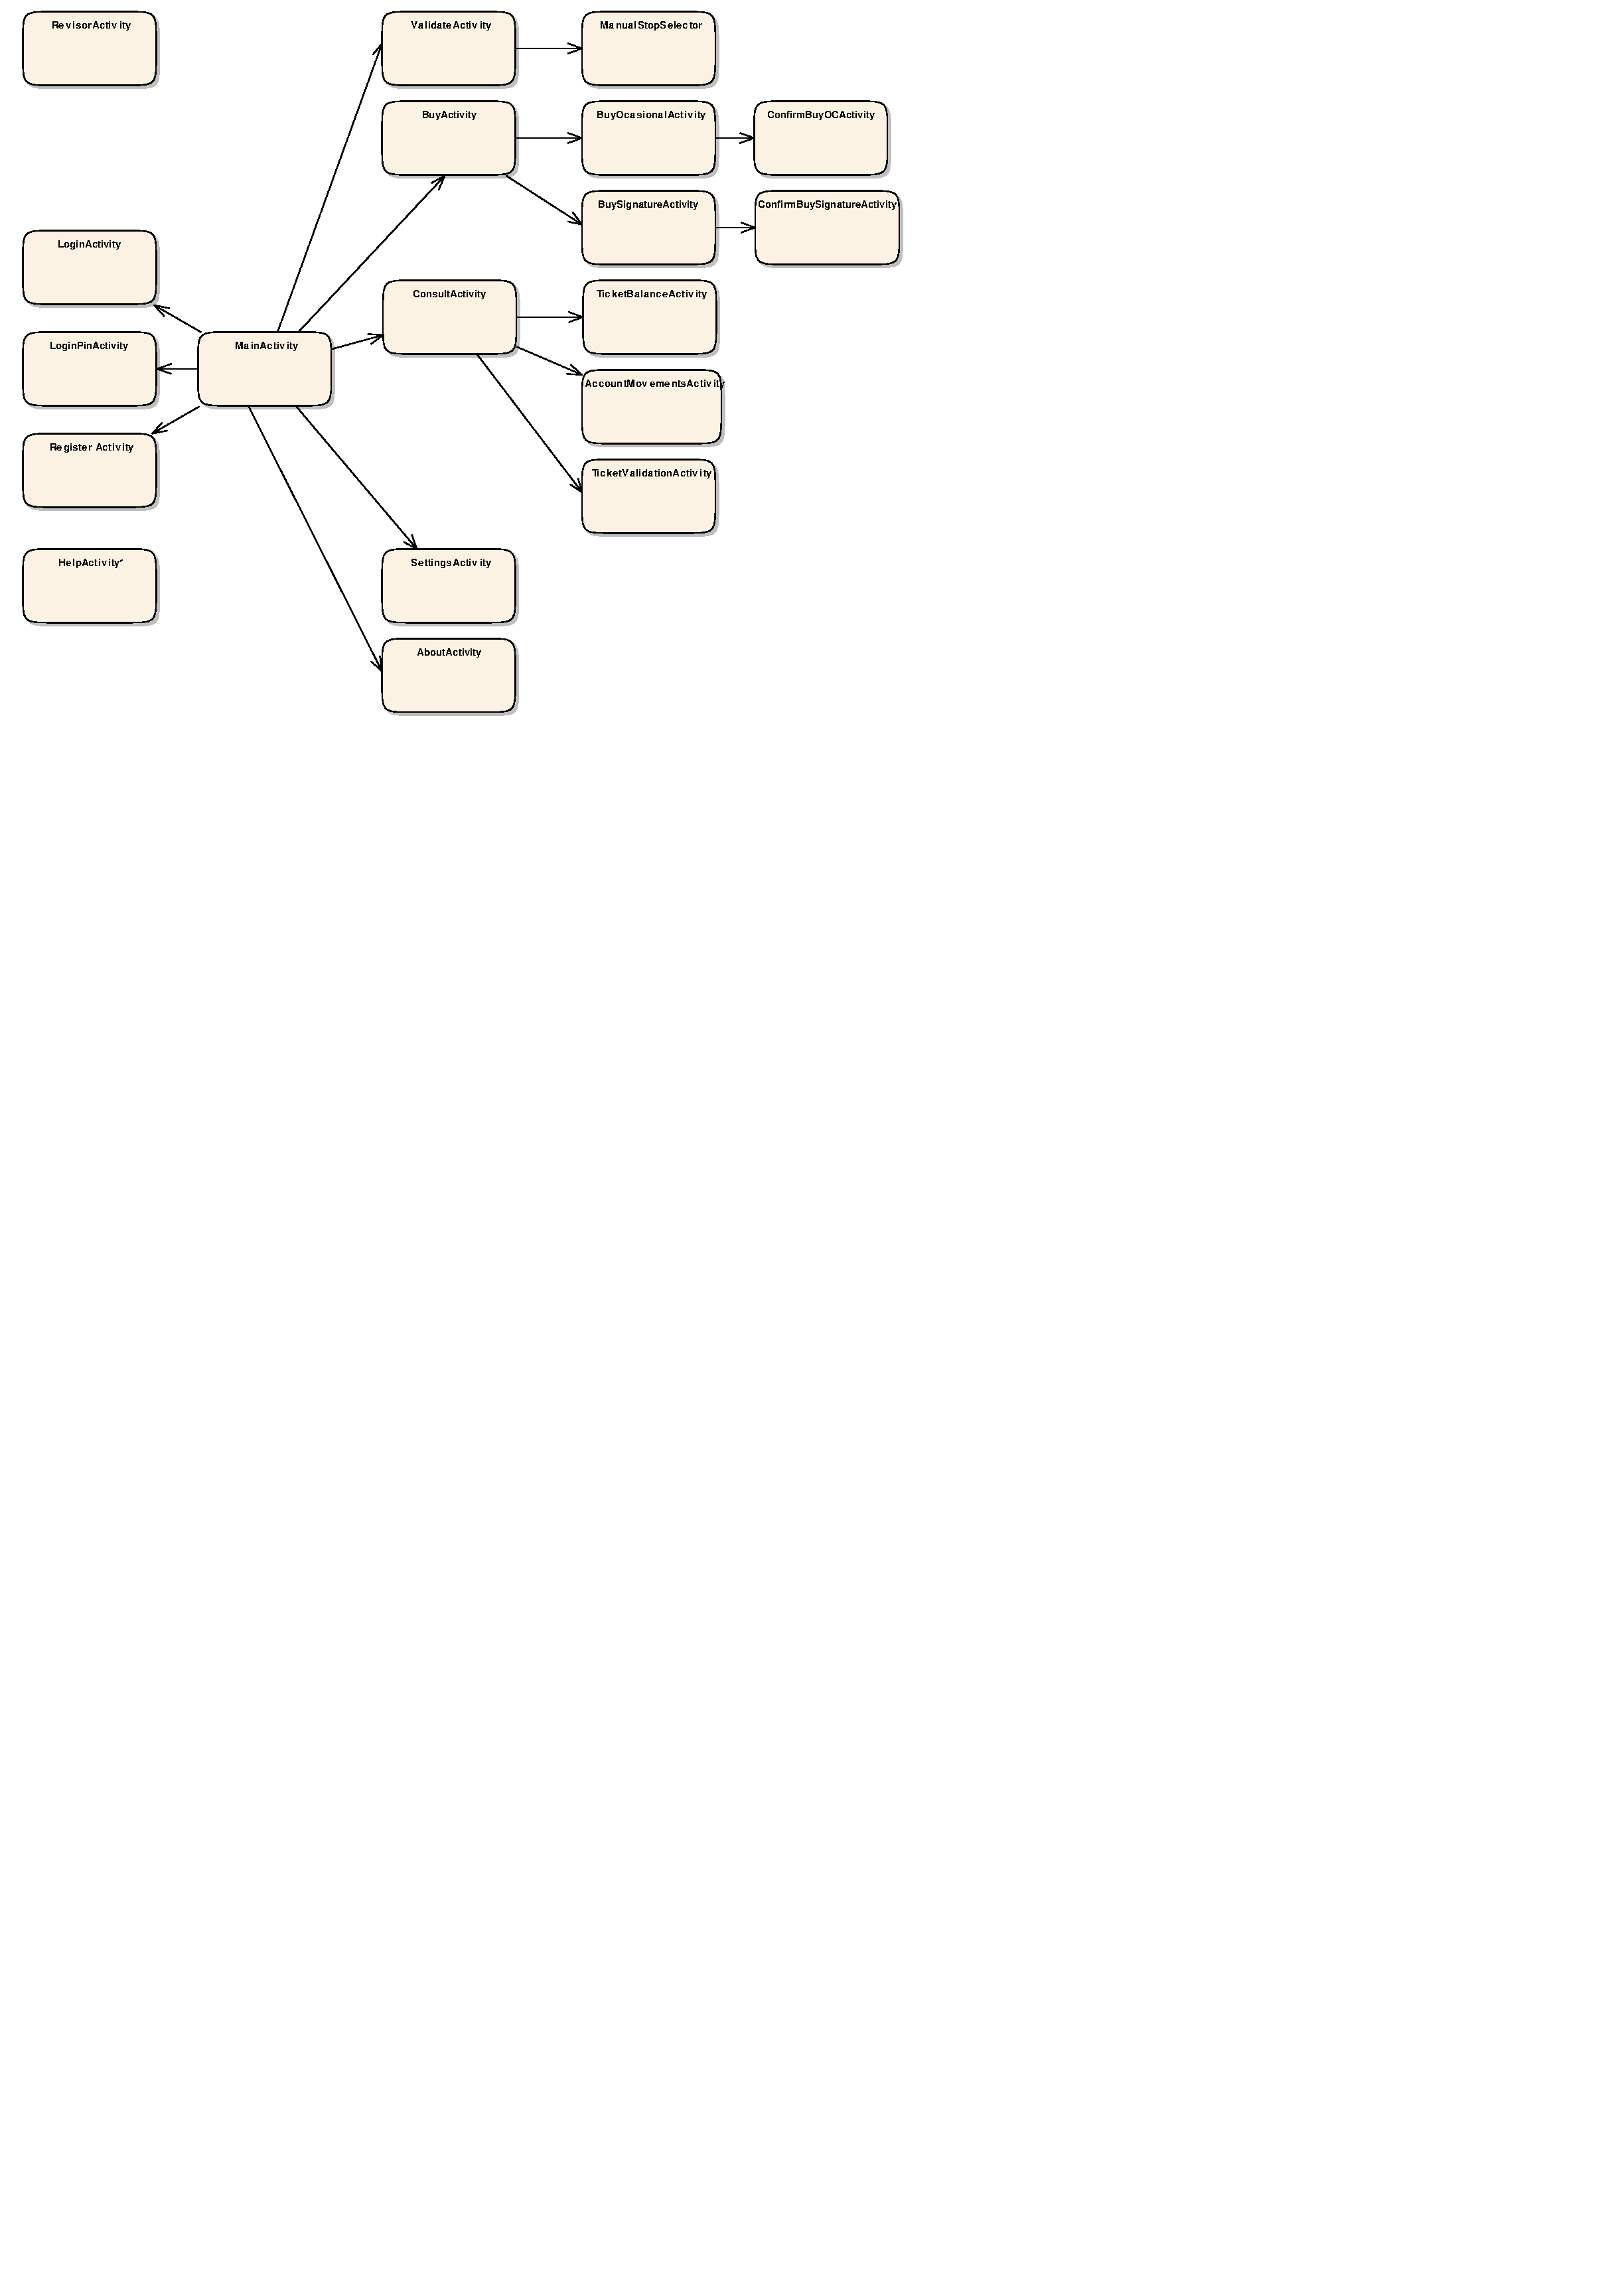
\includegraphics[scale=0.7]{appflow}
    \caption{Diagrama de Atividades}
    \label{fig:appflow}
  \end{center}
\end{figure}

\subsection{Menu Principal}

Este menu é a base da aplicação e serve de lançamento para todas as funcionalidades da mesma. É este o menu a que se acede quando se inicia a aplicação, após autenticação do utilizador. Ver Figura~\ref{fig:menu_principal}.

\subsection{Menu Validação}

Este menu permite efetuar a validação de um título disponível em saldo, para uma determinada paragem e linha. Através dos serviços de localização do dispositivo móvel (GPS e redes móveis), a aplicação tenta calcular a posição atual do utilizador e listar-lhe as paragens que se encontram mais próximas. Caso não seja possível efetuar a localização do utilizador ou esta se encontre errada, o utilizador pode optar por efetuar uma seleção manual da paragem de entrada. Ver Figura~\ref{fig:menu_validacao}. Após a validação surge no ecrã uma mensagem de confirmação, indicando a paragem até à qual o utilizador pode viajar com o título que selecionou, tal como se pode ver na Figura~\ref{fig:confirm_validacao}.

\subsection{Menu Seleção Manual}

Este menu serve para selecionar manualmente a paragem de entrada quando não é possível fazê-lo de forma automática através dos serviços de localização do dispositivo móvel. A sequência de escolha é: Operador, Linha, Paragem. Ver Figura~\ref{fig:menu_manual}.

\subsection{Menu Compra}

Este menu permite ao utilizador iniciar o processo de compra de novos títulos. Para além de apresentar as várias opções de compra, permite também verificar quais os títulos atuais existentes. Deste modo, é fácil verificar se é necessário comprar determinado tipo de título ou se já existe em saldo. Ver Figura~\ref{fig:menu_compra}.

\subsection{Menu Compra Ocasionais}

Este menu permite ao utilizador comprar títulos ocasionais (títulos de viagem ou Andante 24, conforme a seleção no menu anterior), selecionando o número de zonas pretendido, a quantidade (1, 2, 5, 10+1 grátis) e confirmando os dados da compra no menu seguinte. Ver Figura~\ref{fig:menu_compra_oc} e Figura~\ref{fig:confirm_compra_oc}.

\subsection{Menu Compra Assinatura}

Este menu permite ao utilizador comprar uma assinatura mensal, selecionando as zonas pretendidas e confirmando os dados da compra no menu seguinte. Ver Figura~\ref{fig:menu_compra_as} e Figura~\ref{fig:confirm_compra_as}.

\subsection{Menu Consulta}

Este menu é onde o utilizador pode consultar os dados operacionais da sua conta. Para além de consultar o saldo atual de títulos, pode consultar o histórico de operações realizadas na conta e também as validações efetuadas com os seus títulos. Ver Figura~\ref{fig:menu_consulta}.

\subsection{Menu Saldo Títulos}

Este menu permite visualizar o saldo atual de títulos. Neste menu são listados todos os títulos disponíveis para uso imediato, não sendo listada a assinatura do mês seguinte (caso já tenha sido comprada) porque não pode ser usada durante o mês corrente. Ver Figura~\ref{fig:menu_consulta_saldo}.

\subsection{Menu Operações de Conta}

Este menu permite ao utilizador verificar as operações efetuadas na sua conta, quer sejam carregamentos da conta ou compras de títulos. Ver Figura~\ref{fig:menu_operacoes}.

\subsection{Menu Histórico Validações}

Este menu mostra as validações efetuadas pelo utilizador, tanto em títulos ocasionais como na assinatura mensal, conforme a escolha no menu anterior. Ver Figura~\ref{fig:menu_historico} e Figura~\ref{fig:menu_historico2}.

\subsection{Menu Definições}

Este menu permite alterar os dados pessoais do utilizador. Para além disso, permite também fazer \emph{logout} da conta ativa. Ver Figura~\ref{fig:menu_definicoes}.

\subsection{Menu Sobre}

Este menu fornece informação relativa à autoria e desenvolvimento da aplicação MobiPag STCP, bem como a versão atual. Ver Figura~\ref{fig:menu_sobre}.

\subsection{Menu PIN}

Este menu aparece sempre que se inicia a aplicação e permite adicionar uma camada de segurança à aplicação. O PIN do utilizador é definido no registo e pode ser alterado nas Definições. Este método de autenticação surge quando já existe um utilizador com a conta autenticada na aplicação. Para além disso, permite também fazer \emph{logout} da conta ativa. Ver Figura~\ref{fig:menu_login_pin}.

\subsection{Menu Login}

Este menu aparece quando não existe nenhuma conta autenticada na aplicação, permitindo efetuar \emph{login} com o conjunto email/palavra-passe ou então efetuar o registo de um novo utilizador. Ver Figura~\ref{fig:menu_login}.

\subsection{Menu Revisor}

Este menu serve para mostrar informação relativa ao título ativo, quando solicitada pelo revisor autorizado. No caso dos títulos ocasionais, esta informação inclui todas as validações efetuadas com o título em questão, contendo a data e hora, paragem e linha de entrada, bem como o número sequencial da validação. Para além disso, contém informação relativa ao título em uso. Ver Figura~\ref{fig:menu_revisor_oc}. No caso das assinaturas, apenas é apresentada a última validação, mas são apresentados alguns dados pessoais do utilizador, visto a assinatura ser de uso pessoal intransmissível. Para além da informação relativa à assinatura, está também presente o nome e Número de Informação Fiscal do utilizador e uma foto tipo passe. Ver Figura~\ref{fig:menu_revisor_as}.

~\\Para acrescentar alguma segurança e fiabilidade a este menu, foi acrescentado um fundo que varia ao longo do tempo. Tendo como objetivo criar um impacto visual imediato, optou-se por utilizar o código ColorADD, seguidamente detalhado.

\subsubsection{ColorADD}

O código ColorADD é uma inovação mundial, criada pelo designer Miguel Neiva, de um código de cores para daltónicos. Este sistema já se encontra em uso em transportes, hospitais, marcas de lápis, tintas ou cerâmicas. É a primeira ferramenta a procurar diminuir os efeitos de um constrangimento pouco visível: o Daltonismo. O Daltonismo, ou a cegueira da cor, é uma limitação que afeta 10\% da população mundial masculina – aproximadamente 350 milhões de pessoas em todo o mundo. Esta limitação, de condição hereditária, é transmitida através do cromossoma X e cria ao seu portador grandes constrangimentos ao nível da integração social e profissional.
\\Desenvolvido com base nas três cores primárias representadas através de símbolos gráficos, o código ColorADD assenta no conceito de “adição de cores”, permitindo ao daltónico relacionar os símbolos e facilmente identificar toda a paleta. O Branco e o Preto surgem para orientar as tonalidades claras e escuras. O código torna-se num “jogo mental” simples e fácil de memorizar e aplicar em situações do dia-a-dia. \cite{coloradd}
\\Para uma visualização completa das cores, ver Anexo~\ref{coloradd}.

\subsection{Menu Ajuda}

Este é um menu contextual, fornecendo informação acerca do menu atual. O objetivo é esclarecer, de forma clara, qualquer dúvida que possa surgir durante a utilização da aplicação. Ver Figura~\ref{fig:menu_ajuda}.

\begin{figure}[t]
  \begin{center}
    \leavevmode
    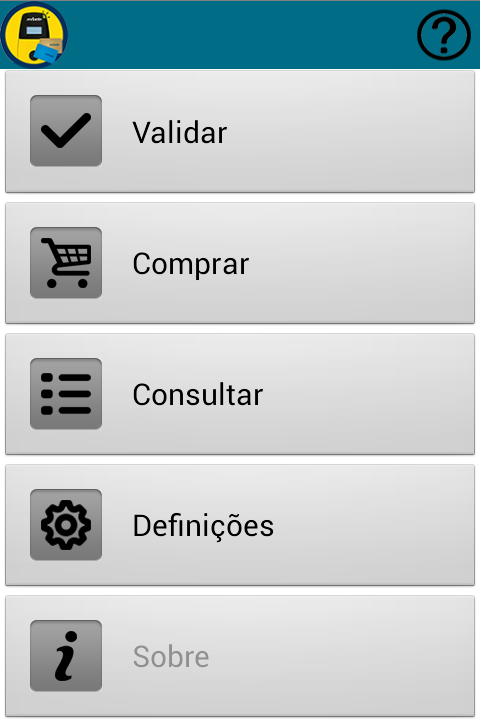
\includegraphics[scale=0.40]{menu_principal}
    \caption{Menu Principal}
    \label{fig:menu_principal}
  \end{center}
\end{figure}

\begin{figure}[ht]
\begin{minipage}[b]{0.45\linewidth}
\centering
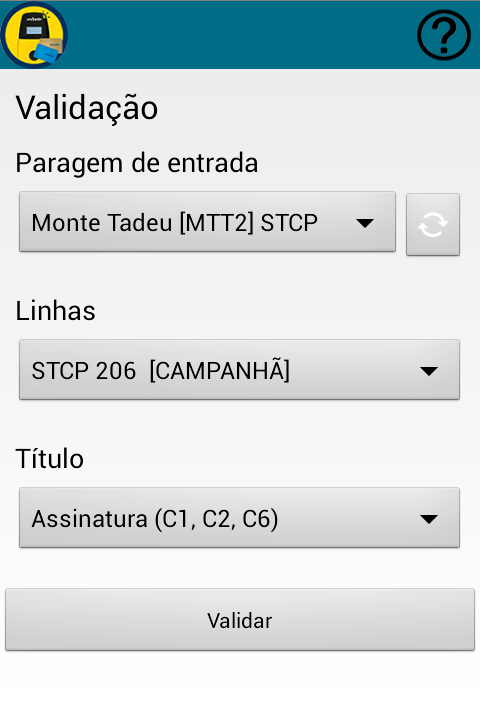
\includegraphics[width=\textwidth]{menu_validacao}
    \caption{Menu Validação}
    \label{fig:menu_validacao}
\end{minipage}
\hspace{0.5cm}
\begin{minipage}[b]{0.45\linewidth}
\centering
    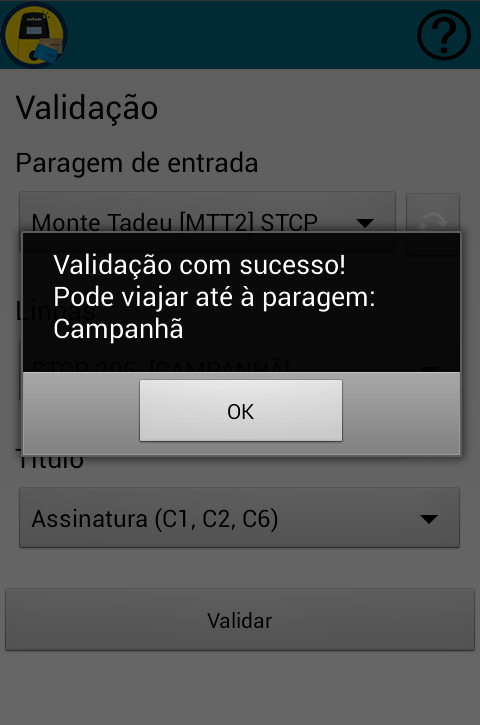
\includegraphics[width=\textwidth]{confirm_validacao}
    \caption{Confirmação Validação}
    \label{fig:confirm_validacao}
\end{minipage}
\end{figure}

\begin{figure}[ht]
\begin{minipage}[b]{0.45\linewidth}
\centering
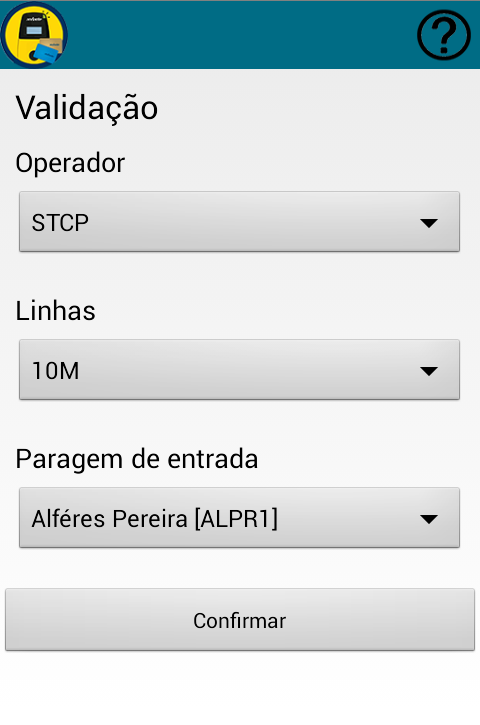
\includegraphics[width=\textwidth]{menu_manual}
    \caption{Menu Seleção Manual}
    \label{fig:menu_manual}
\end{minipage}
\hspace{0.5cm}
\begin{minipage}[b]{0.45\linewidth}
\centering
    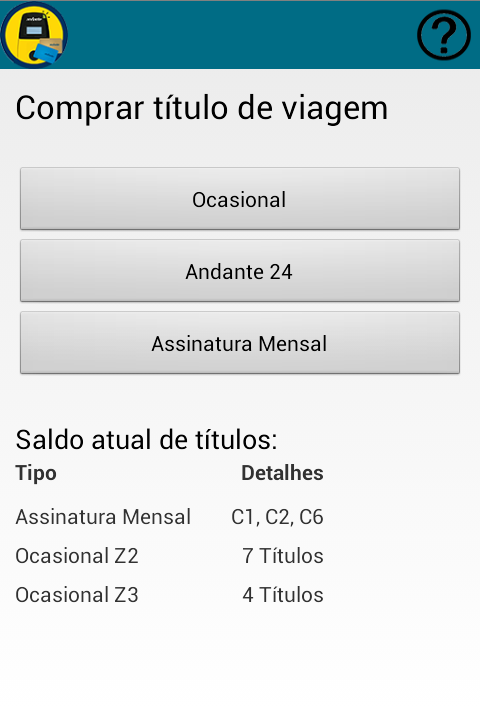
\includegraphics[width=\textwidth]{menu_compra}
    \caption{Menu Compra}
    \label{fig:menu_compra}
\end{minipage}
\end{figure}

\begin{figure}[ht]
\begin{minipage}[b]{0.45\linewidth}
\centering
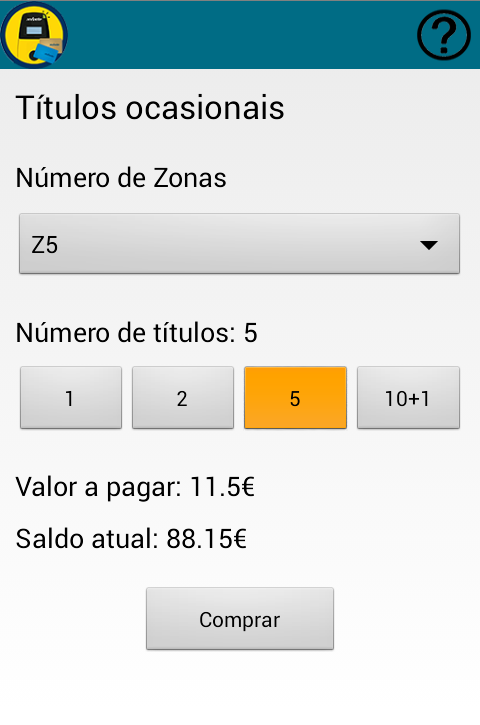
\includegraphics[width=\textwidth]{menu_compra_oc}
    \caption{Menu Compra Ocasionais}
    \label{fig:menu_compra_oc}
\end{minipage}
\hspace{0.5cm}
\begin{minipage}[b]{0.45\linewidth}
\centering
    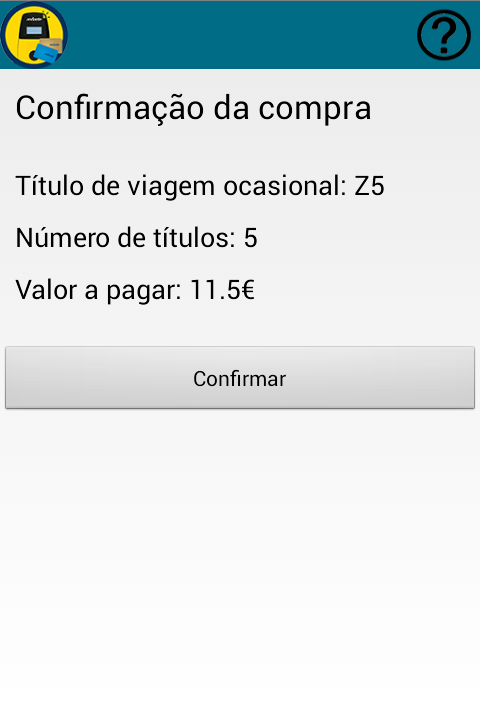
\includegraphics[width=\textwidth]{confirm_compra_oc}
    \caption{Confirm. Compra Ocasionais}
    \label{fig:confirm_compra_oc}
\end{minipage}
\end{figure}

\begin{figure}[ht]
\begin{minipage}[b]{0.45\linewidth}
\centering
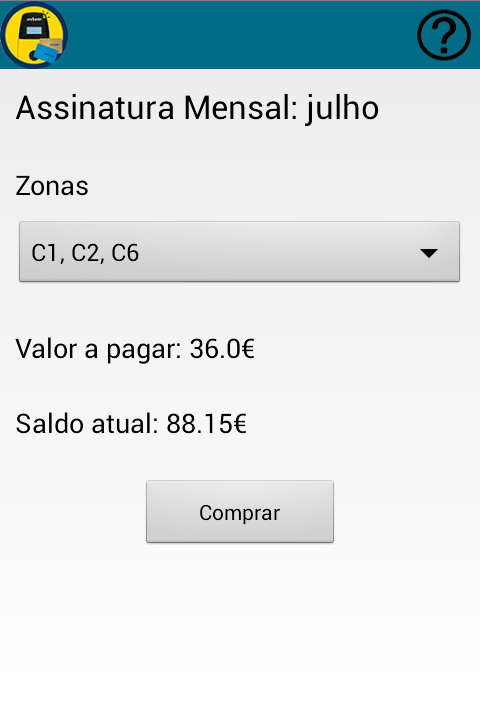
\includegraphics[width=\textwidth]{menu_compra_as}
    \caption{Menu Compra Assinatura}
    \label{fig:menu_compra_as}
\end{minipage}
\hspace{0.5cm}
\begin{minipage}[b]{0.45\linewidth}
\centering
    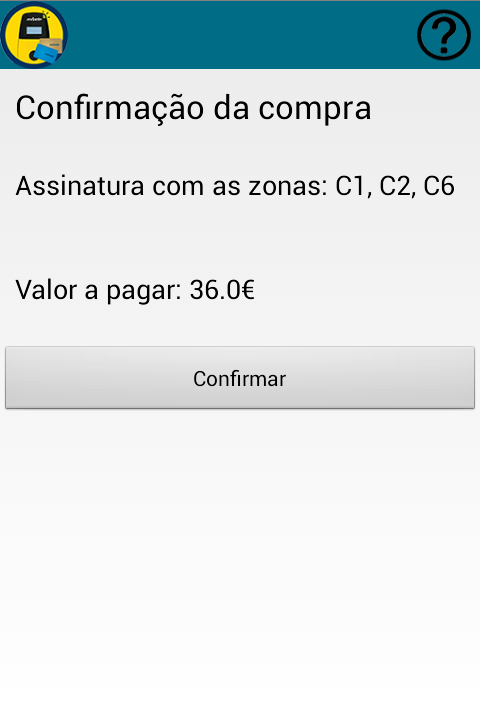
\includegraphics[width=\textwidth]{confirm_compra_as}
    \caption{Confirm. Compra Assinatura}
    \label{fig:confirm_compra_as}
\end{minipage}
\end{figure}

\begin{figure}[ht]
\begin{minipage}[b]{0.45\linewidth}
\centering
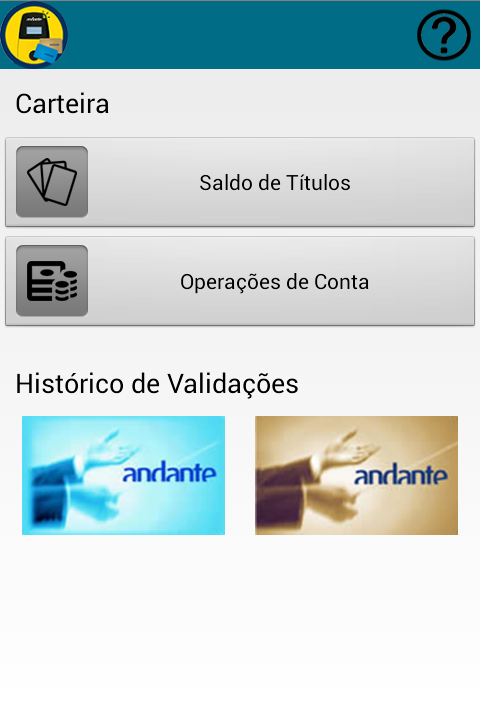
\includegraphics[width=\textwidth]{menu_consulta}
    \caption{Menu Consulta}
    \label{fig:menu_consulta}
\end{minipage}
\hspace{0.5cm}
\begin{minipage}[b]{0.45\linewidth}
\centering
    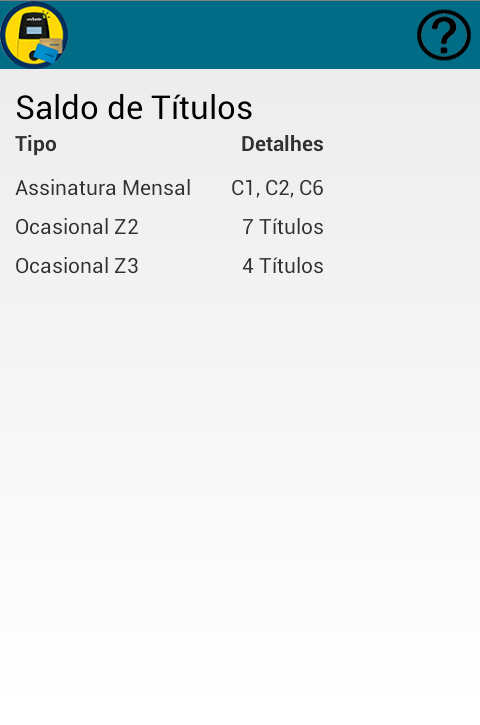
\includegraphics[width=\textwidth]{menu_consulta_saldo}
    \caption{Menu Saldo Títulos}
    \label{fig:menu_consulta_saldo}
\end{minipage}
\end{figure}

\begin{figure}[ht]
\begin{minipage}[b]{0.31\linewidth}
\centering
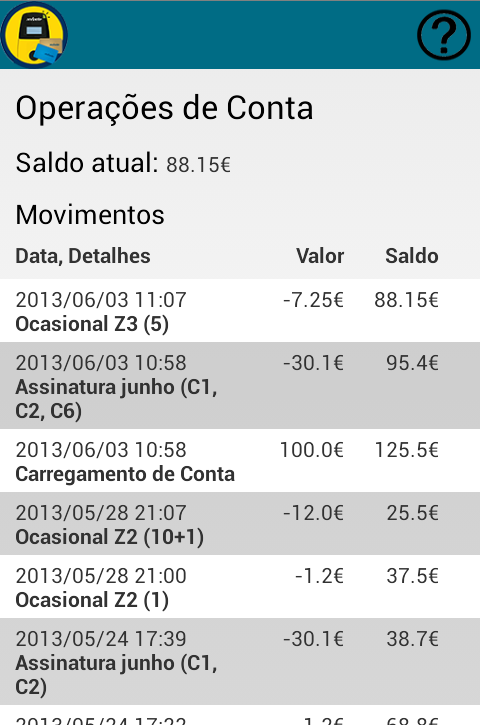
\includegraphics[width=\textwidth]{menu_operacoes}
    \caption{Menu Operações de Conta}
    \label{fig:menu_operacoes}
\end{minipage}
\hspace{0.25cm}
\begin{minipage}[b]{0.31\linewidth}
\centering
    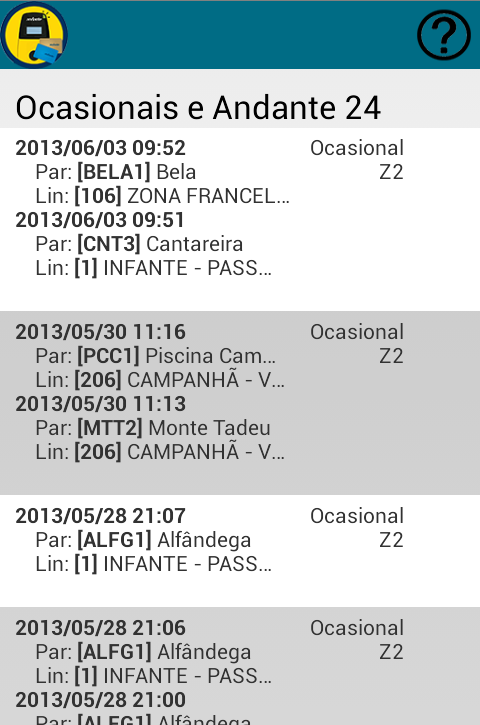
\includegraphics[width=\textwidth]{menu_historico}
    \caption{Menu Histórico Validações Ocasionais}
    \label{fig:menu_historico}
\end{minipage}
\hspace{0.25cm}
\begin{minipage}[b]{0.31\linewidth}
\centering
    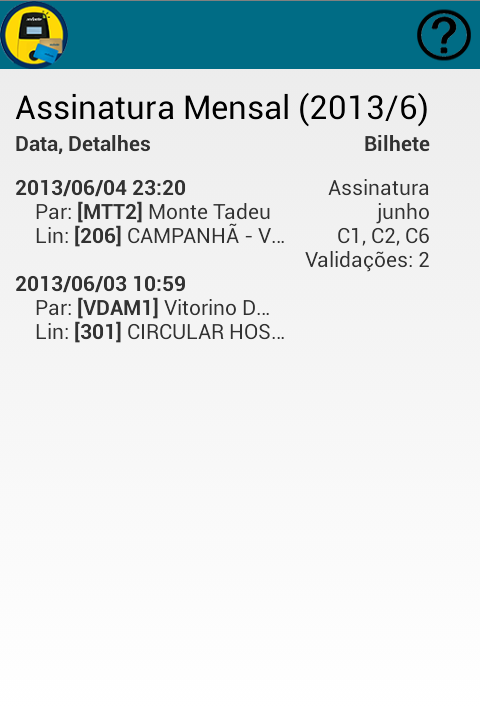
\includegraphics[width=\textwidth]{menu_historico2}
    \caption{Menu Histórico Validações Assinatura}
    \label{fig:menu_historico2}
\end{minipage}
\end{figure}

\begin{figure}[ht]
\begin{minipage}[b]{0.45\linewidth}
\centering
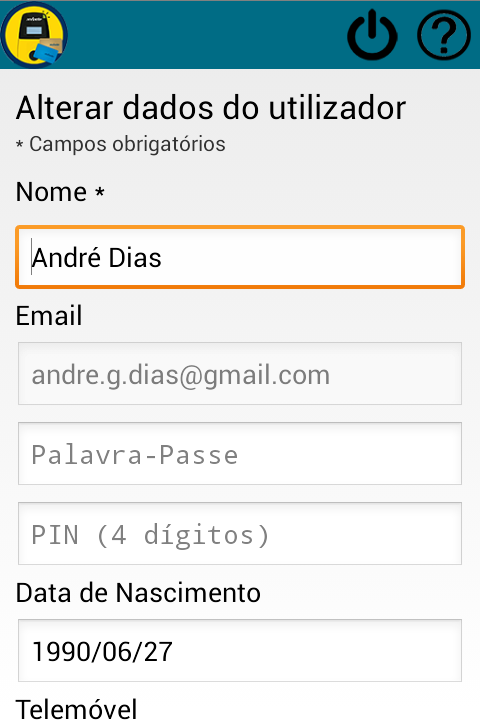
\includegraphics[width=\textwidth]{menu_definicoes}
    \caption{Menu Definições}
    \label{fig:menu_definicoes}
\end{minipage}
\hspace{0.5cm}
\begin{minipage}[b]{0.45\linewidth}
\centering
    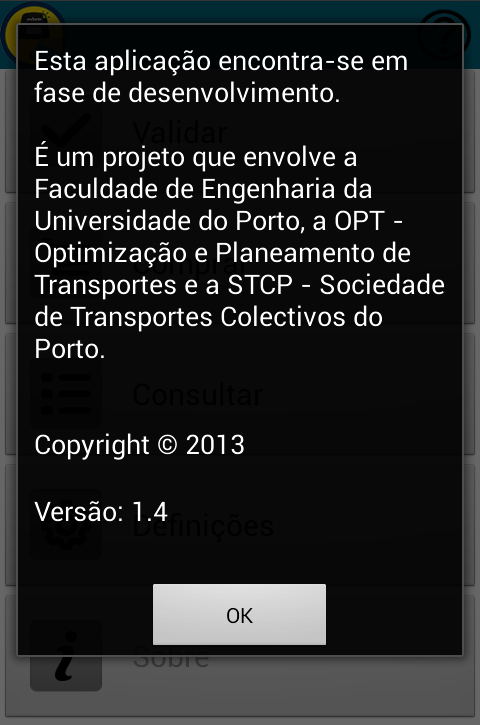
\includegraphics[width=\textwidth]{menu_sobre}
    \caption{Menu Sobre}
    \label{fig:menu_sobre}
\end{minipage}
\end{figure}

\begin{figure}[ht]
\begin{minipage}[b]{0.45\linewidth}
\centering
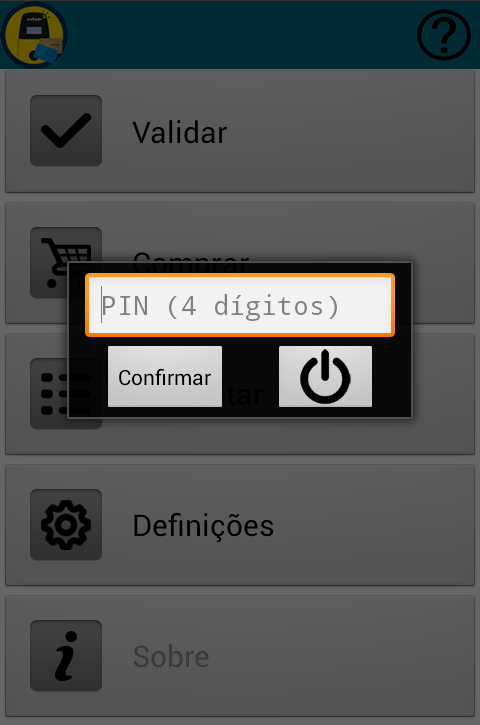
\includegraphics[width=\textwidth]{menu_login_pin}
    \caption{Menu PIN}
    \label{fig:menu_login_pin}
\end{minipage}
\hspace{0.5cm}
\begin{minipage}[b]{0.45\linewidth}
\centering
    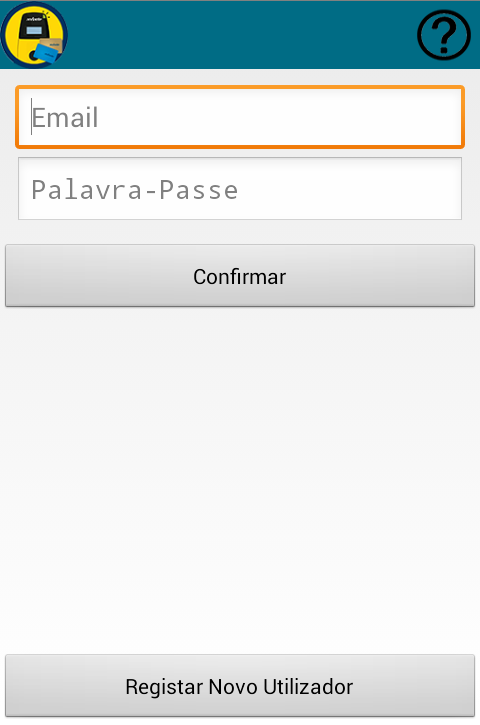
\includegraphics[width=\textwidth]{menu_login}
    \caption{Menu Login}
    \label{fig:menu_login}
\end{minipage}
\end{figure}

\begin{figure}[ht]
\begin{minipage}[b]{0.45\linewidth}
\centering
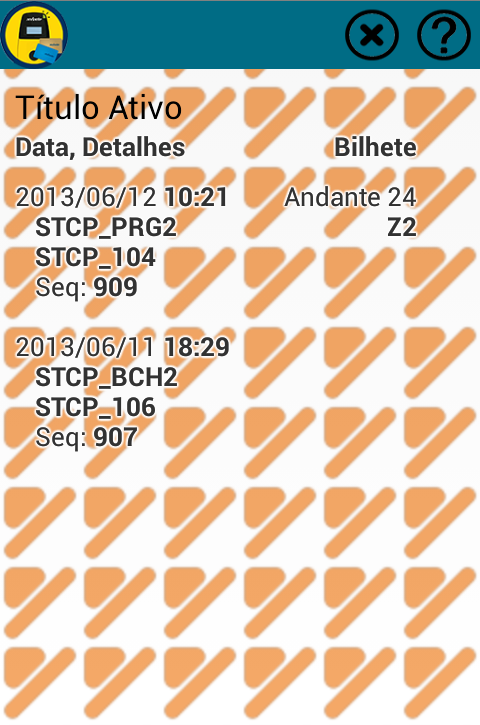
\includegraphics[width=\textwidth]{menu_revisor_oc}
    \caption{Menu Revisor}
    \label{fig:menu_revisor_oc}
\end{minipage}
\hspace{0.5cm}
\begin{minipage}[b]{0.45\linewidth}
\centering
    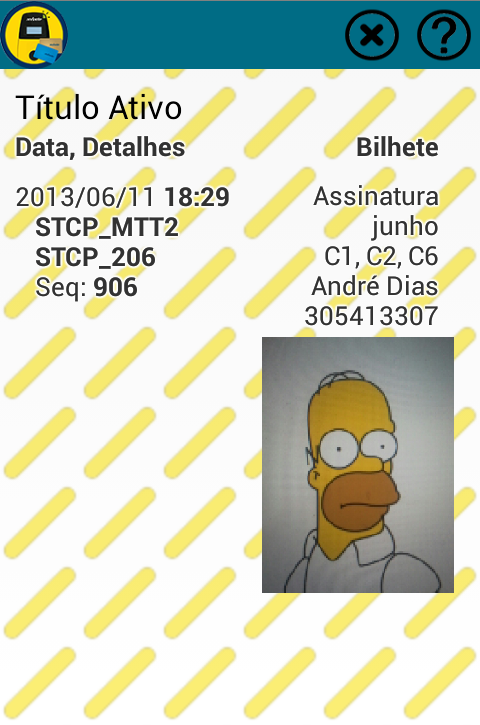
\includegraphics[width=\textwidth]{menu_revisor_as}
    \caption{Menu Revisor}
    \label{fig:menu_revisor_as}
\end{minipage}
\end{figure}

\begin{figure}[t]
  \begin{center}
    \leavevmode
    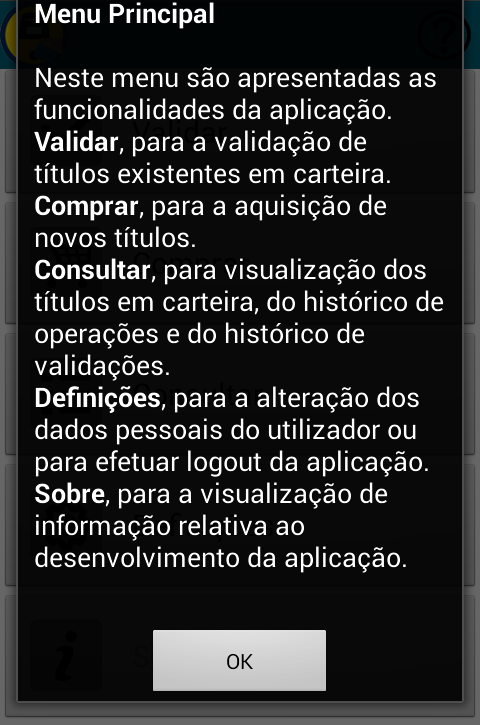
\includegraphics[scale=0.40]{menu_ajuda}
    \caption{Menu Ajuda}
    \label{fig:menu_ajuda}
  \end{center}
\end{figure}